\documentclass[11pt]{article}
\usepackage{graphicx,listings}
\graphicspath{ {./images/} }
\title{\textbf{IoT 2023 Challenge 3}}
\author{
  Pasquale Castiglione\\
	\texttt{10657816}
  \and
  Lorenzo Campana\\
  \texttt{10605775}
}
\date{}
\begin{document}
\maketitle

\section*{RadioRoute.h}
In the header file, the data structures for the messages and for the routing table were defined.
\begin{figure}[h]
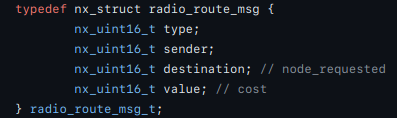
\includegraphics[scale=0.5]{msg.png}
\caption{Message data structure}
\end{figure}
\begin{figure}[h]
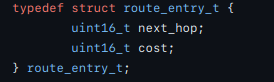
\includegraphics[scale=0.5]{entry.png}
\caption{Entry of the routing table}
\end{figure}

\section*{RadioRouteC.nc}
\subsection*{Variables} 
\begin{itemize}
	\item{\texttt{waiting\_packet:}} Stores a packet that is waiting for a routing table update before it can be sent. It allows the code to delay the sending of the packet until a valid route is obtained.
	\item{\texttt{waiting\_address:}} Stores the destination address of a packet that is waiting for a routing table update before it can be sent.
	\item{\texttt{locked:}} Controls the sending of packets to avoid overlapping transmissions. When a packet needs to be sent, the ``locked" variable is checked. If it is set to ``TRUE", it means that a packet transmission is already in progress, and the sending is aborted. It is later set back to ``FALSE" when the sending is completed.
	\item{\texttt{msg\_counter:}} Keeps track of the number of messages received by a node.
	\item{\texttt{codice\_persona:}} Array containg the codice persona of the leader.

\end{itemize}
\subsection*{Functions}
\begin{itemize}
	\item{\texttt{initializeRoutingTable:}} Initializes the routing table.
	\item{\texttt{getRoutingEntry:}} Retrieves a routing entry from a routing table based on a given destination address
	\item{\texttt{addRoutingEntry:}} Adds or updates an entry to the routing table. 
	\item{\texttt{dbgPacketInfo:}} Prints debug information about packets.
\end{itemize}
\subsection*{Boot}
At the boot of a node, the routing table is created and the radio module is started. When the radio module has finished the process of starting, a five seconds timer is started for the node `1'.
\subsection*{Send Event}
The sending of a message is implemented in the 	\texttt{actual\_send} function.
Before the sending of a message, the variable \texttt{locked} is evaluated in order to check if a packet is already being sent or not.
If the module is not locked, it proceeds with sending the packet. It first checks the routing table to determine the next hop for the packet's destination. If a routing entry is found, it uses the next hop as the address for sending. If no routing entry is found, it uses the provided address parameter as the destination address.
In case of data message with null entry in the routing table, \texttt{waiting\_packet} and \texttt{waiting\_address} are set and a routing request is sent in broadcast.
\subsection*{Receive Event}
Received messages are handled according to their type:
\begin{itemize}
	\item{\textbf{Data Message}}\\
		Checks if the message is intended for the current node. If not, it checks if a route to the destination is present in its routing table. If a route is present then it forwards the message to the next hop.
	\item{\textbf{Route Request}}\\
		If the receiver node is the intended destination of a route request or if the node has a non empty entry in the routing table, then it answers back sending a \texttt{Route Reply} broadcast message.
		Otherwise it broadcast again the route request message to its neighbors.
		
	\item{\textbf{Route Reply}}\\
		When a \texttt{Route Reply} is received the nodes check their routing table and they update them if the received cost for the destination is lower than the stored one.
		Also, the nodes check weather there is a \texttt{waiting\_packet} with a \texttt{waiting\_address} equals to the updated entry destination address.
		In this case, it proceeds with the packet forwarding to the updated next hop.
\end{itemize}
\section*{Led Control}
The LED index is calculated based on the \texttt{msg\_counter} variable and the \texttt{codice\_persona} array. The \texttt{msg\_counter} is incremented each time a packet is received, and it is used to select the digit in a round-robin cycle from the \texttt{codice\_persona} array. The digit is then used to determine the LED index by taking its modulo with 3. At this point the led status is toggled using \texttt{Leds.ledToggle()}
\end{document}
